\documentclass[12pt,a4paper]{article}
\usepackage {ngerman}
\usepackage{helvet}
\renewcommand{\familydefault}{\sfdefault}
\usepackage{amsmath}
\usepackage{amsfonts}
\usepackage{amssymb}
\usepackage{graphicx}
\usepackage[left=3cm,right=2.5cm,top=2.5cm,bottom=2.5cm]{geometry}
\usepackage[headsepline,footsepline]{scrlayer-scrpage}
\usepackage{microtype}
\usepackage{pdfpages}
\usepackage{color}
\usepackage[hyphens]{url}
\usepackage{lastpage}
\usepackage[colorlinks=true,urlcolor=blue,linkcolor=black]{hyperref}
\hyphenpenalty=9999
\exhyphenpenalty=9999
\setheadsepline{.5pt}
\setfootsepline{.5pt}
\setlength{\headheight}{20pt} 
\pagestyle{scrheadings}
\clearscrheadfoot
\clearscrheadings
\clearscrplain
\author{Felix Kuschel
	\and Manuel Starz}
\title{Entwicklung einer Smart Home Zentrale auf Basis eines RaspberryPI}
% Kopf- & Fußzeilen... werden nicht angezeigt, wenn \chapter{} verwendet wird. Stattdessen \section{} verwenden...
% Kopfzeile
\ihead{
\includegraphics[width=0.2\textwidth]{its_logo.pdf}}
\chead{}
\ohead{\textsc{Kuschel \& Starz}}
% Fußzeile
\ifoot{\textsc{FTI2 2020/2021}}
\cfoot{}
\ofoot{\textsc{Seite \pagemark\:von \pageref{LastPage}}} % Achtung, Muss 2 mal comilieren, sonst Fehler^^
\date{-}
\definecolor{quotetext}{rgb}{.35,.35,.35} %{1,.64,0}
\begin{document}
	% Titelseite. Basierend auf https://de.wikibooks.org/wiki/LaTeX/_Eine_Titelseite_erstellen
	\begin{titlepage}
		\centering
		
\includegraphics[width=0.5\textwidth]{its_logo.pdf}\par\vspace{1cm}
		% {\scshape\LARGE it.schule stuttgart \par}
		\vspace{1cm}
		{\scshape\Large Technikerarbeit\par}
		\vspace{1.5cm}
		{\huge\bfseries\scshape Entwicklung einer Smart Home Zentrale auf Basis eines RaspberryPI\par}
		\vspace{2cm}
		{\Large Felix \textsc{Kuschel} \& Manuel \textsc{Starz}\par}
		\vfill
		Betreut durch\par
		~Matthias \textsc{Kohler}

		\vfill

		% Bottom of the page
		{\large \today\par}
	\end{titlepage}
	% Inhaltsverzeichnis
	\tableofcontents
	\newpage
	\section*{Erklärung}
	Wir versichern, dass die vorliegende Abschlussarbeit von uns selbstständig angefertigt und nur die angegebenen Hilfsmittel benutzt wurden. An Stellen, die dem Wortlaut oder dem Sinne nach anderen Werken entnommen sind, haben wir dies durch die Angabe der Quellen kenntlich gemacht.
	\vspace{2cm}	
	\\
	\noindent\rule{7cm}{.4pt}\hfill\rule{7cm}{.4pt}\par
	\noindent Datum, Ort \hfill Felix Kuschel
	\vspace{2cm}	
	\\
	\noindent\rule{7cm}{.4pt}\hfill\rule{7cm}{.4pt}\par
	\noindent Datum, Ort \hfill Manuel Starz
	\newpage
	\section{Vorwort}
 	\subsection{Einleitung}
 	Bei dieser Ausarbeitung handelt es sich um die Abschlussarbeit zur Weiterbildung zum staatlich geprüften Techniker in der Fachrichtung Informationstechnik. Diese Arbeit basiert auf dem in den zwei Jahren erlernten Stoffs sowie selbst erarbeiteten Kenntnissen und dient zur Feststellung des Erreichen des Fortbildungsziels.
 	\subsection{Projektrahmen}
 	Das Projekt zur Erstellung einer Smart Home Zentrale wurde von uns, Felix Kuschel und Manuel Starz, durchgeführt. Der Projektzeitraum war vom 1. September 2020 bis zum 30.03.2021 angesetzt. Es stand zur Umsetzung des Projekts ein unterrichtsfreier Tag pro Woche zur Verfügung.\par
 	Des weiteren wurden die in dem Zeitraum zur Verfügung stehenden Ferien zur Umsetzung des Projekts genutzt. Die Projektbetreuung erfolgten seitens der Schule durch Herr Matthias Kohler. Da das Projekt nicht in Zusammenarbeit mit einem Unternehmen durchgeführt wurde, gibt es keine weiteren Betreuer. Die Materialkosten für die im Projekt genutzte Hardware wurde von den uns selbst getragen.
 	\subsection{Aufgabenstellung}
 	Das Projekt ist aus dem Zusammenschluss der Abschlussarbeitsideen von uns, Felix Kuschel und Manuel Starz, entstanden und wurde mit Rücksprache mit dem betreuenden Lehrer entwickelt.\par
 	 Durch die große Verfügbarkeit von Smart Home Geräten und den zahlreichen Standards der Anbieter entschlossen wir uns, eine einfache und leicht zu replizierende Lösung zu entwickeln, die Smart Home Geräte mehrerer Hersteller miteinander verknüpft und so die Notwendigkeit mehrerer verschiedener sogenannter Hubs zu eliminieren. \par
 	Des weiteren soll das Gerät noch über einen Touchscreen steuerbar sein und die Werte der verbundenen Smart Home Geräte anzeigen. Dies umfasst unter anderem den Status von Leuchtmitteln, die Werte von Thermostaten sowie den Zustand von Tür- und Fensterkontakten. Die genaue Aufgabenstellung kann dem abgegebenen Lastenheft im Anhang entnommen werden.
 	\subsection{Zusatzinformationen}
 	Die Rohdaten des Projekts wurden der Einfachheit in einem GIT-Projekt zusammengefasst. Dadurch konnten die Durchführenden unabhängig voneinander an dem Projekt und der Dokumentation arbeiten.\par
 	Der Link zu dem Projekt lautet:\\
 	\textbf{https://github.com/Pharias/TAR}\par
 	Ursprünglich wurde für die Verwendung des schulinternen GIT verwendet. Dies stand zum Zeitpunkt der Erstellung der Dokumentation allerdings nicht zur Verfügung, weshalb eine Alternative genutzt wurde.
 	\subsection{Definition Smart Home Zentrale}
 	\begin{figure}[htb]
 		\centering
 		\begin{minipage}[t]{0.3\linewidth}
 			\centering
 			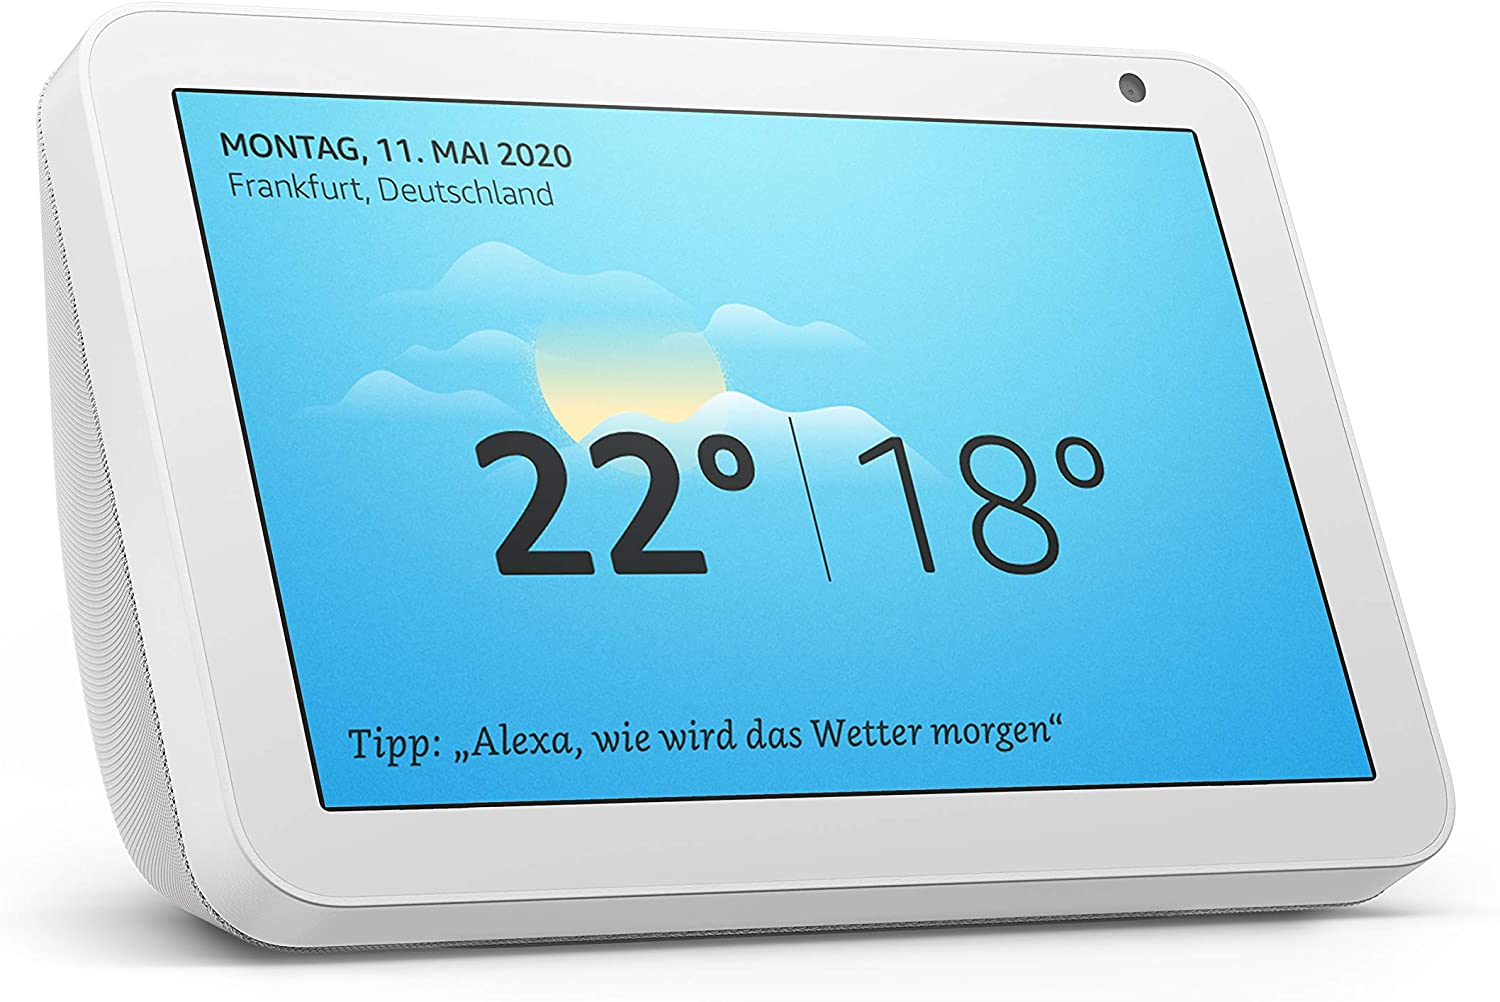
\includegraphics[width=0.7\textwidth]{alexa_echo_show8.jpg}
 			\caption[Amazon Alexa Echo Show 8]{Amazon Alexa Echo Show 8}
 			\label{fig:alexa-echo-show8}
 		\end{minipage}
 		\hfill
 		\begin{minipage}[t]{0.3\linewidth}
 			\centering
 			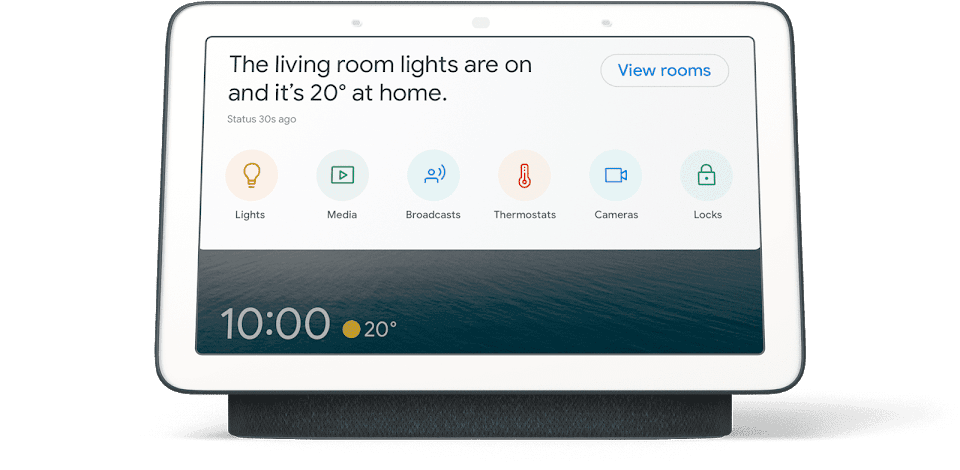
\includegraphics[width=0.7\textwidth]{google_nest_hub.png}
 			\caption[Google Nest Hub]{Google Nest Hub}
 			\label{fig:google-nest-hub}
 		\end{minipage}
 		\hfill
 		\begin{minipage}[t]{0.3\linewidth}
 			\centering
 			\includegraphics[width=0.7\textwidth]{glancr_smart_mirror.jpeg}
 			\caption[Glancr Smart Mirror]{Glancr Smart Mirror}
 			\label{fig:glancr-smart-mirror}
 		\end{minipage}
 	\end{figure}
 	\textbf{Smart Home Zentralen}, auch \textbf{Smart Hubs} oder \textbf{Smart Mirrors} genannt, sind Geräte, die als zentraler Knotenpunkt in einem Smart Home Netzwerk sitzen und dort Informationen verarbeiten, weiterleiten und darstellen können.\par
 	Diese Geräte werden von den meisten Herstellern mit und ohne Bildschirm geliefert, um entweder ein neues Smart Home aufzubauen oder ein bestehendes Smart Home zu erweitern. 
 	\begin{quote}
 	\color{quotetext}
 		Bei einem Smart-Home-Hub handelt es sich um eine schlaue Zentrale, durch die all deine intelligenten Geräte miteinander vernetzt werden – und dadurch erst wirklich ihren gesamten Leistungsumfang ausschöpfen.\footnote{Li (2017): Was ist ein Smart-Home-Hub? Alles über die intelligente Zentrale}
 	\end{quote}
 	
 	\newpage
	% Hier den Rest eintragen...
	% Folgend erst mal der allgemeine Aufbau nach dem einen Beispiel, das ich in Telegram geteilt hab...
	\section{Zielsetzung}
	Als Ziel für das Projekt war ein funktionsfähiges Smart Home Hub mit Zigbee-Anbindung auf Basis eines Raspberry Pi 4 geplant. Im Laufe des Projekts kam dann noch eine Erweiterungskarte für den Raspberry Pi, ein sog. Raspberry Pi HAT, hinzu, welcher aber aufgrund der vorliegenden Lage mit der COVID-19-Pandemie und den damit verbundenen Liefer- und Zollschwierigkeiten verworfen wurde. Die Planung des HAT ist daher nur rudimentär und nicht vollständig, kann aber bei Bedarf nach Beenden des Projekts durchgeführt werden. Das Smart Home Hub in seiner Grundfunktion soll in der Lage sein, die mit ihm verbundenen Geräte über den Zigbee-Standard anzusteuern. Darüber sollte die Möglichkeit einer Erweiterung mit einem Sprachassistenten gegeben sein.\par
	\subsection{Konzeption}
	Zu Beginn des Projekts haben wir uns gemeinsam auf Nachforschung begeben und uns bereits vorhandene Open-Source-Lösungen im Bereich Smart Home angeschaut. Dabei sind wir neben dem Smart Mirror GLANCR auch auf die Gesamtlösung homeassistant.io sowie openHAB gestoßen. Darauf hin haben wir ein Grundkonzept in unserem Lastenheft zusammengefasst und dieses in Absprache mit unserem Betreuungslehrer, Herr Kohler, ausgearbeitet.\par
	Nach Abgabe des Lastenhefts haben wir uns dann an die Beschaffung der unserer Meinung nach nötigen Komponenten für das Projekt gemacht.
	\subsection{Anforderungen und gewünschte Features}
	Die Anforderungen an das Projekt lauteten demnach wie folgt:
	\begin{itemize}
		\item Anbindung von ZigBee-fähigen Endgeräten
		\item Steuerung der angebundenen Endgeräte
		\item Übermittlung der Zustände der angebundenen Geräte an z.B. ein Smartphone
	\end{itemize}
	Diese Anforderungen lassen sich mit einem Raspberry Pi und einem Zigbee-USB-Stick realisieren. Darüber hinaus waren von unserer Seite noch folgende Features gewünscht:
	\begin{itemize}
		\item Ein- und Ausgabe über einen Touch-Bildschirm
		\item Einbindung eines Sprachassistenten zur Steuerung der eingebundenen Endgeräte
	\end{itemize}
	Nach Fortschritt des Projekts kam bei einer Rücksprache mit unserem Projektbetreuer die Idee auf, einen Raspberry Pi Hat speziell für das Projekt zu entwickeln. Dieser sollte die Hardware des Projekts falls möglich auf einer Platine vereinen, die dann auf den Raspberry Pi aufgesteckt werden konnte.\par
	Diese Erweiterungsplatine sollte folgende Eigenschaften besitzen:
	\begin{itemize}
		\item ZigBee-Controller und Antenne
		\item NFC-Controller und Antenne
		\item RGB-LED zur Statusanzeige
		\item Anschluss für Lüfter
		\item Sensoren für:
		\begin{itemize}
			 \item Luftfeuchtigkeit
			 \item Temperatur
			 \item Luftdruck
		\end{itemize}
		\item Pins zum Anschluss an Versuchsaufbau für Laborgebrauch
	\end{itemize}
	Die Erweiterungsplatine wurde aber wie zuvor aufgrund der aktuellen Pandemie-Situation und den damit verbundenen Beschaffungsschwierigkeiten verworfen.
	Darauf wurde dann klar, dass eine Erstellung eines Installationsskripts für den Raspberry Pi eine sinnvolle Ergänzung der Projektarbeit wäre. Zusätzlich haben wir ein Gehäuse für die Hardware geplant, um das Endprodukt so wertiger gestalten zu können.
	\newpage
	\section{Herangehensweise}
	Nach Festlegung der Anforderungen haben wir uns dann mit der Beschaffung und der Einrichtung der benötigten Materialien gemacht. Hierfür haben wir zum Teil bereits vorhandene Hardware, z.B. den Raspberry Pi 4 mit weiteren Komponenten wie dem Touch-Bildschirm und den Lautsprechern sowie dem Mikrofon ergänzt.
	\subsection{Hardware}
	\subsection{Software}
	\section{Zeitplan}
		\begin{figure}[htb]
			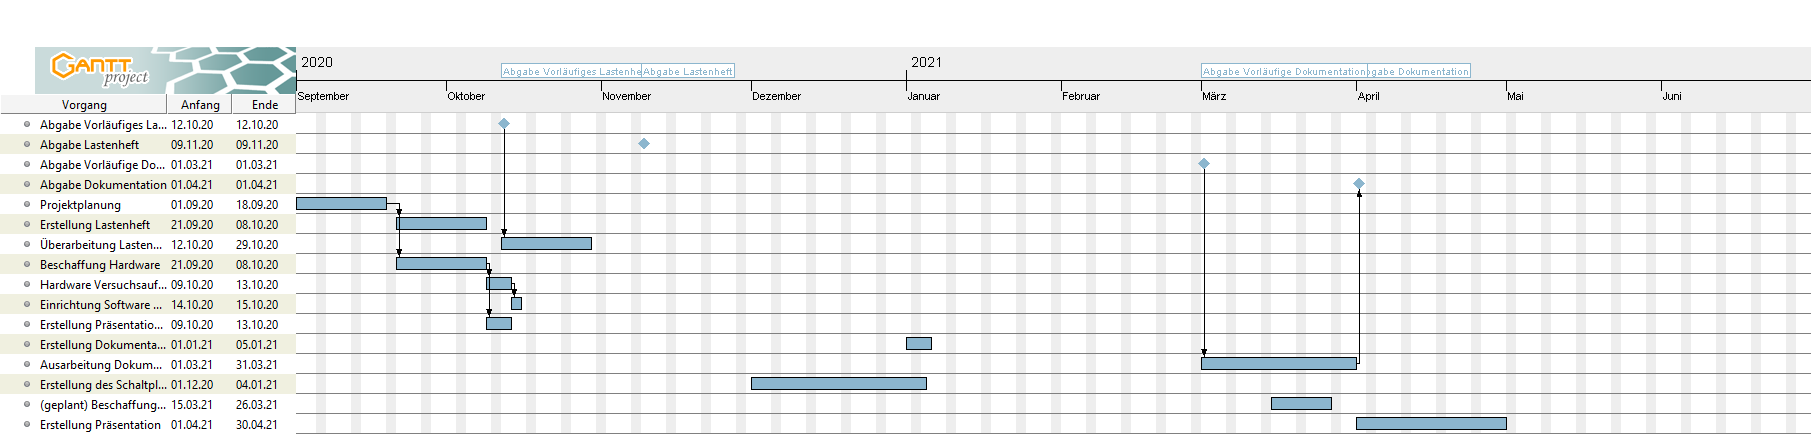
\includegraphics[width=0.9\textwidth]{TAR_FKMS_20202021.png}
			\caption[gantt-Diagramm des Projektablaufs]{gantt-Diagramm des Projektablaufs}
 			\label{fig:gantt-diagramm}
 		\end{figure}
	\section{Komplettübersicht}
	\section{Hardware}
	\subsection{Raspberry Pi 4}
	\subsection{Aufbau des Prototypen}
	\subsection{Gehäuse}
	\subsection{Erstellung des RPi-HATs}
	\section{Software}
	\subsection{Überblick}
	\subsection{MQTT-Broker}
	\subsection{HomeAssistant}
	\subsection{MyCroft}
	\subsection{HAT-Programm}
	\section{Epilog \& Fazit}
	\newpage	
 	\section{Quellen}
 	% Quellen auflisten
 	\subsection{Dokumentationsquellen}
 	Quellen, die in Fußnoten innerhalb dieser Dokumentation erwähnt wurden.
 	\begin{itemize}
 		\item Li (2017): Was ist ein Smart-Home-Hub? Alles über die intelligente Zentrale\\ {\url{https://www.otto.de/updated/ratgeber/erklaert-was-ist-ein-smart-home-hub-80634/}}
 	\end{itemize}
 	\subsection{Verwendete Software}
 	\begin{tabular}{|l|l|l|}
 	\hline 
 	\textbf{Software} & \textbf{Verwendung} & \textbf{Version} \\ 
 	\hline 
 	Raspberry Pi OS & Betriebssystem und Oberfläche für Hardware & 5.4 \\ 
 	\hline 
 	Home Assistant & Betriebssystem und Oberfläche für Smart Home & 5.12 \\ 
 	\hline 
 	KiCad EDA & Erstellung von Schaltplan und Gerber-Datei des Hats & 5.1.8 \\ 
 	\hline 
 	TexMaker & Erstellung der Dokumentation & 5.0.4 \\ 
 	\hline 
 	Fusion360 & Erstellung von Gehäusemodell & 2.0.9849 \\ 
 	\hline
 	CURA & Erstellung von G-Code für 3D-Drucker & 4.7 \\ 
 	\hline
 	GanttProject & Erstellung von Gantt-Diagrammen & 3.0.3 \\ 
 	\hline
 	\end{tabular} 
 	\subsection{Verwendete Hardware}
 	\begin{tabular}{|l|l|l|}
 	\hline
 	\textbf{Hardware} & \textbf{Verwendung} & \textbf{Version} \\
 	\hline
 	Raspberry Pi & Hauptplatine für die  & Version 4B (8GB)\\
 	 & Smart Home Zentrale &\\
 	\hline
 	CC2531 Zigbee USB & USB-Stick mit ZigBee-Chip & Rev 2.4\\
 	Stick mit Firmware& & \\
 	\hline
 	Sunfounder 10.1  & Bildschirm und Input für & Unbekannt\\
 	Touch Screen & die Smart Home Zentrale & \\
 	 \hline
 	\end{tabular}
 	\section{Anhang}
 	% Lastenheft, andere Dokumente etc...
 	\subsection{Lastenheft}
 	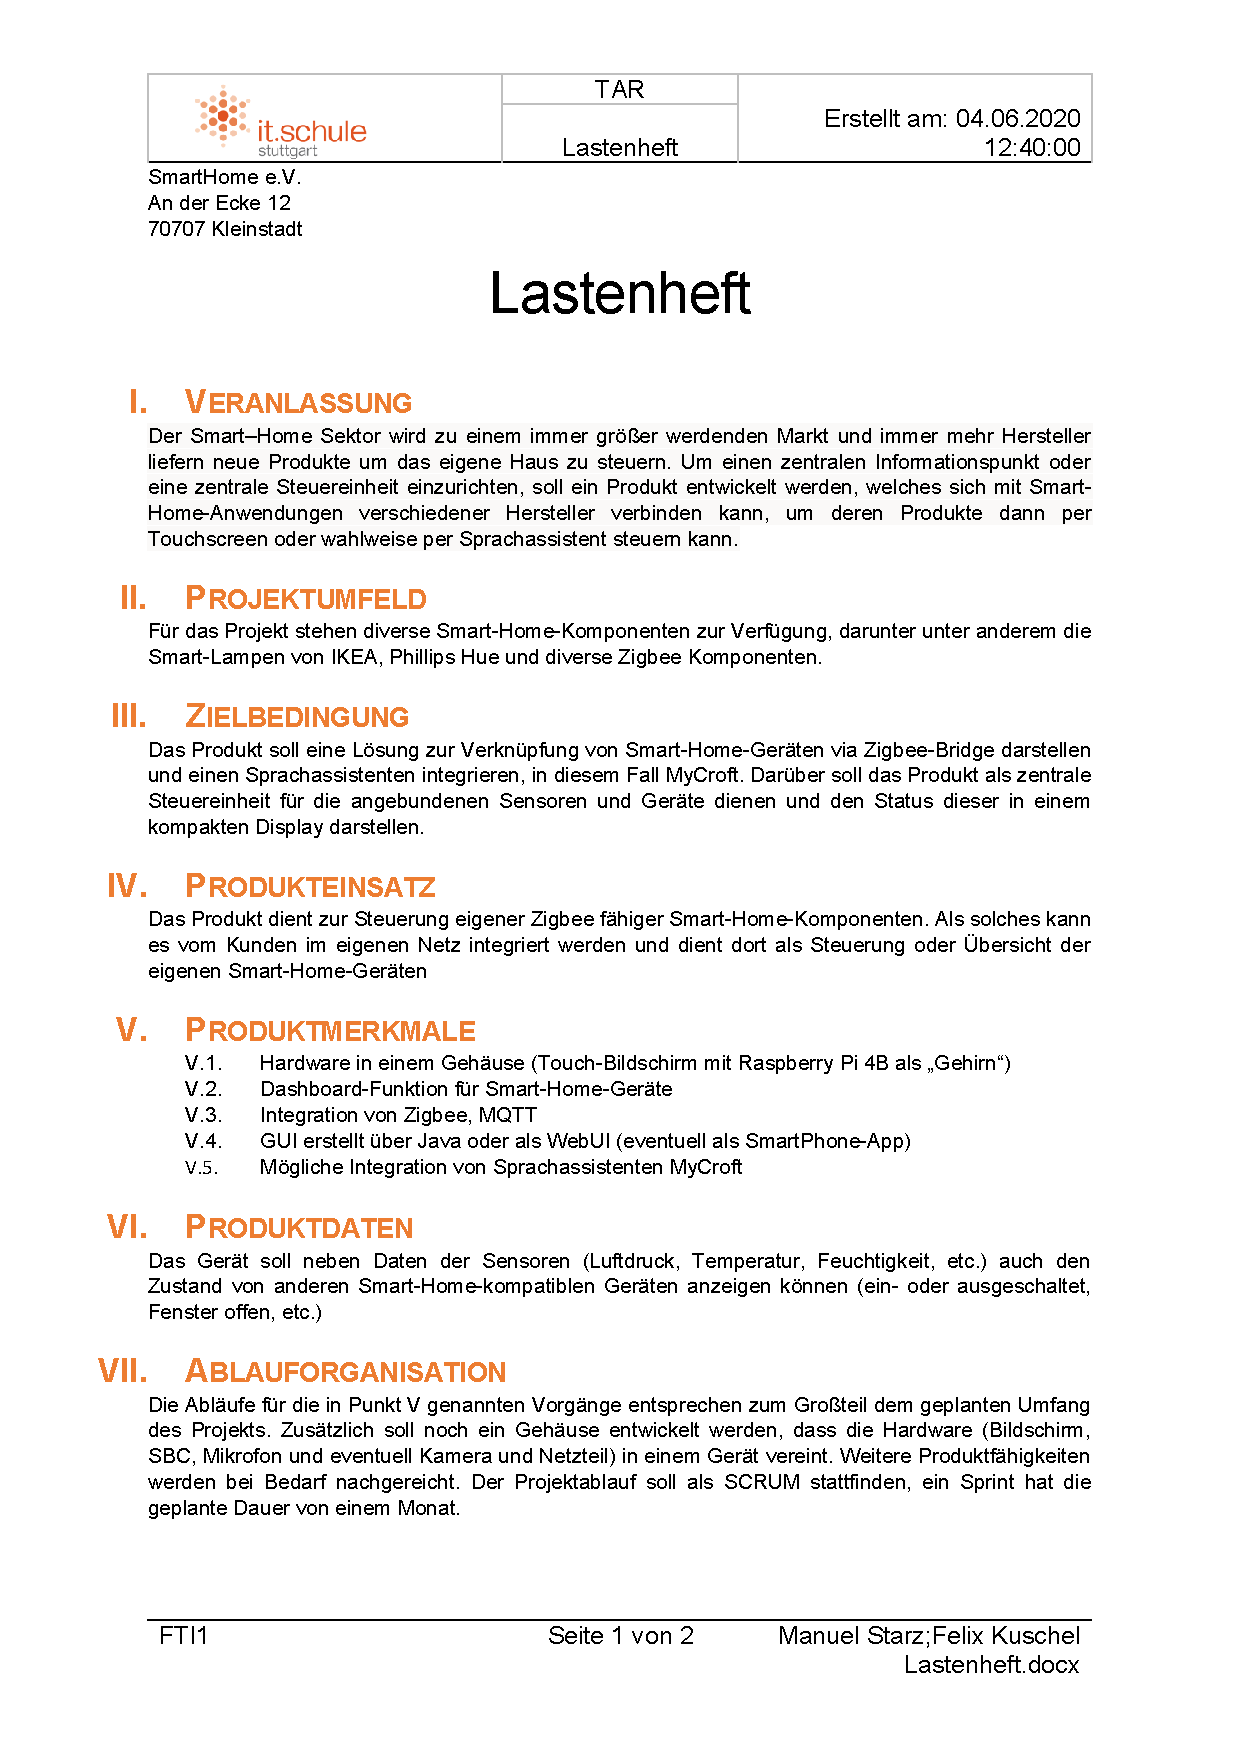
\includegraphics[width=0.98\textwidth, page=1]{lastenheft.pdf}
 	\newpage
 	\includegraphics[width=0.98\textwidth, page=2]{lastenheft.pdf}
 	\newpage
 	\subsection{Hardware-Dokumentationen}
 	Durch den Umfang der einzelnen Dokumentationen hier nur eine Auflistung der Dokumentationen mit dem Link zu den PDF im GIT-Projekt bzw. den Herstellerseiten.
 	\begin{itemize}
 		\item Raspberry Pi:\\ {\url{https://www.raspberrypi.org/documentation/hardware/raspberrypi/bcm2711/rpi_DATA_2711_1p0.pdf}}
 		\item MiFare MFRC522:\\ {\url{https://www.nxp.com/docs/en/data-sheet/MFRC522.pdf}}
 		\item CC2531 ZigBee SoC:\\ {\url{https://www.ti.com/lit/ds/symlink/cc2531.pdf}}
 		\item ATmega128RFA1-ZU:\\ {\url{https://ww1.microchip.com/downloads/en/DeviceDoc/Atmel-8266-MCU_Wireless-ATmega128RFA1_Datasheet.pdf}}
 	\end{itemize}
 	\newpage
 	\listoffigures
\end{document}
